\chapter{Исследовательская часть}

В данном разделе приводится анализ производительности разработанного программного комплекса. Поскольку система реализует алгоритмы трёхмерной визуализации средствами центрального процессора без использования аппаратного ускорения видеокарты, критически важным является исследование временных затрат на генерацию кадра и выявление факторов, влияющих на быстродействие.

\section{Цель и задачи исследования}

\textbf{Целью} исследования является оценка зависимости времени генерации одного кадра изображения от коэффициента масштабирования сцены.

В ходе исследования решались следующие \textbf{задачи}:
\begin{enumerate}
	\item внедрение в программный код средств профилирования для измерения чистого времени рендеринга.
	\item проведение серии замеров при плавном изменении коэффициента масштабирования от начального значения до максимального.
	\item анализ полученной зависимости и оценка эффективности алгоритмов отсечения невидимой геометрии.
\end{enumerate}

\section{Технические характеристики стенда}

Экспериментальное исследование проводилось на ноутбуке со следующей аппаратной и программной конфигурацией:

\begin{itemize}
	\item \textbf{Центральный процессор (CPU):} AMD Ryzen 7 8845HS, тактовая частота 3.8 ГГц;
	\item \textbf{Оперативная память (RAM):} 32 ГБ;
	\item \textbf{Операционная система:} Microsoft Windows 11 (64-bit);
	\item \textbf{Среда выполнения:} Интерпретатор Python 3.13.
\end{itemize}

Для обеспечения стабильности и точности замеров были выполнены следующие действия:
\begin{enumerate}
	\item подключение ноутбука к источнику бесперебойного питания;
	\item завершение всех остальных пользовательских приложений, не использующихся для замеров времени.
\end{enumerate}

Замеры времени выполнялись с использованием системного таймера с точностью до одной десятой миллисекунды.

\section{Методика проведения исследования}

Для получения данных использовалась следующая методика:
\begin{enumerate}
	\item камера устанавливалась в начальное положение (вид сверху); исходный коэффициент масштабирования (\texttt{Scale}) задавался равным увеличению изображения в \textbf{40 раз};
	\item производилось плавное увеличение коэффициента масштабирования от \textbf{40-кратного} до \textbf{150-кратного} увеличения, при этом фиксировалось время генерации каждого кадра;
	\item для исключения случайных выбросов, замеры для каждого коэффициента масштабирования проводились \textbf{10 раз}, а полученные значения усреднялись.
\end{enumerate}


\section{Результаты исследования}

В таблице \ref{tab:render_time} приведены полные результаты замеров времени отрисовки кадра при плавном изменении коэффициента масштабирования от 40-кратного до 150-кратного увеличения с шагом 2.0. Графическая интерпретация зависимости представлена на рисунке \ref{fig:research_graph}.

\sisetup{output-decimal-marker={,}} % Необходимо, чтобы числа выводились с запятой в качестве разделителя

\sisetup{output-decimal-marker={,}, group-digits=false} % Устанавливаем запятую как десятичный разделитель и отключаем группировку разрядов

\begin{table}[H]
	\captionsetup{justification=raggedleft, singlelinecheck=false}
	\caption{Зависимость времени генерации кадра от коэффициента масштабирования}
	\label{tab:render_time}
	\small % Увеличенный шрифт (больше, чем \scriptsize)
	\centering
	% S[table-format=3.1]: Scale (e.g., 150.0)
	% S[table-format=4.1]: Время (мс) (e.g., 1272.9)
	% S[table-format=1.2]: FPS (e.g., 1.55)
	\begin{tabular}{|S[table-format=3.1]|S[table-format=4.1]|S[table-format=1.2]||S[table-format=3.1]|S[table-format=4.1]|S[table-format=1.2]|}
		\hline
		\textbf{Scale} & \textbf{Время (мс)} & \textbf{FPS} & \textbf{Scale} & \textbf{Время (мс)} & \textbf{FPS} \\ \hline
		40.0 & 646.8 & 1.55 & 96.0 & 1104.7 & 0.90 \\ \hline
		42.0 & 678.4 & 1.47 & 98.0 & 1084.6 & 0.92 \\ \hline
		44.0 & 707.2 & 1.41 & 100.0 & 1024.9 & 0.98 \\ \hline
		46.0 & 739.5 & 1.35 & 102.0 & 1020.7 & 0.98 \\ \hline
		48.0 & 772.9 & 1.29 & 104.0 & 1073.9 & 0.93 \\ \hline
		50.0 & 811.6 & 1.23 & 106.0 & 1115.4 & 0.90 \\ \hline
		52.0 & 855.3 & 1.17 & 108.0 & 1046.1 & 0.96 \\ \hline
		54.0 & 836.7 & 1.19 & 110.0 & 1007.8 & 0.99 \\ \hline
		56.0 & 948.2 & 1.05 & 112.0 & 1021.3 & 0.98 \\ \hline
		58.0 & 1062.4 & 0.94 & 114.0 & 1145.4 & 0.87 \\ \hline
		60.0 & 1014.6 & 0.99 & 116.0 & 1020.8 & 0.98 \\ \hline
		62.0 & 1051.8 & 0.95 & 118.0 & 1048.3 & 0.95 \\ \hline
		64.0 & 1056.4 & 0.95 & 120.0 & 1012.6 & 0.99 \\ \hline
		66.0 & 1132.7 & 0.88 & 122.0 & 991.7 & 1.01 \\ \hline
		68.0 & 1058.9 & 0.94 & 124.0 & 1055.8 & 0.95 \\ \hline
		70.0 & 1131.5 & 0.88 & 126.0 & 1054.2 & 0.95 \\ \hline
		72.0 & 1139.8 & 0.88 & 128.0 & 978.3 & 1.02 \\ \hline
		74.0 & 1246.3 & 0.80 & 130.0 & 913.8 & 1.09 \\ \hline
		76.0 & 1260.7 & 0.79 & 132.0 & 947.5 & 1.06 \\ \hline
		78.0 & 1218.4 & 0.82 & 134.0 & 993.2 & 1.01 \\ \hline
		80.0 & 1253.6 & 0.80 & 136.0 & 971.8 & 1.03 \\ \hline
		82.0 & 1272.9 & 0.79 & 138.0 & 966.5 & 1.03 \\ \hline
		84.0 & 1208.7 & 0.83 & 140.0 & 957.3 & 1.04 \\ \hline
		86.0 & 1179.3 & 0.85 & 142.0 & 947.2 & 1.05 \\ \hline
		88.0 & 1154.8 & 0.87 & 144.0 & 917.5 & 1.09 \\ \hline
		90.0 & 1142.3 & 0.88 & 146.0 & 887.9 & 1.12 \\ \hline
		92.0 & 1146.7 & 0.87 & 148.0 & 937.4 & 1.07 \\ \hline
		94.0 & 1078.4 & 0.93 & 150.0 & 971.1 & 1.03 \\ \hline
	\end{tabular}
\end{table}

\begin{figure}[H]
	\centering
	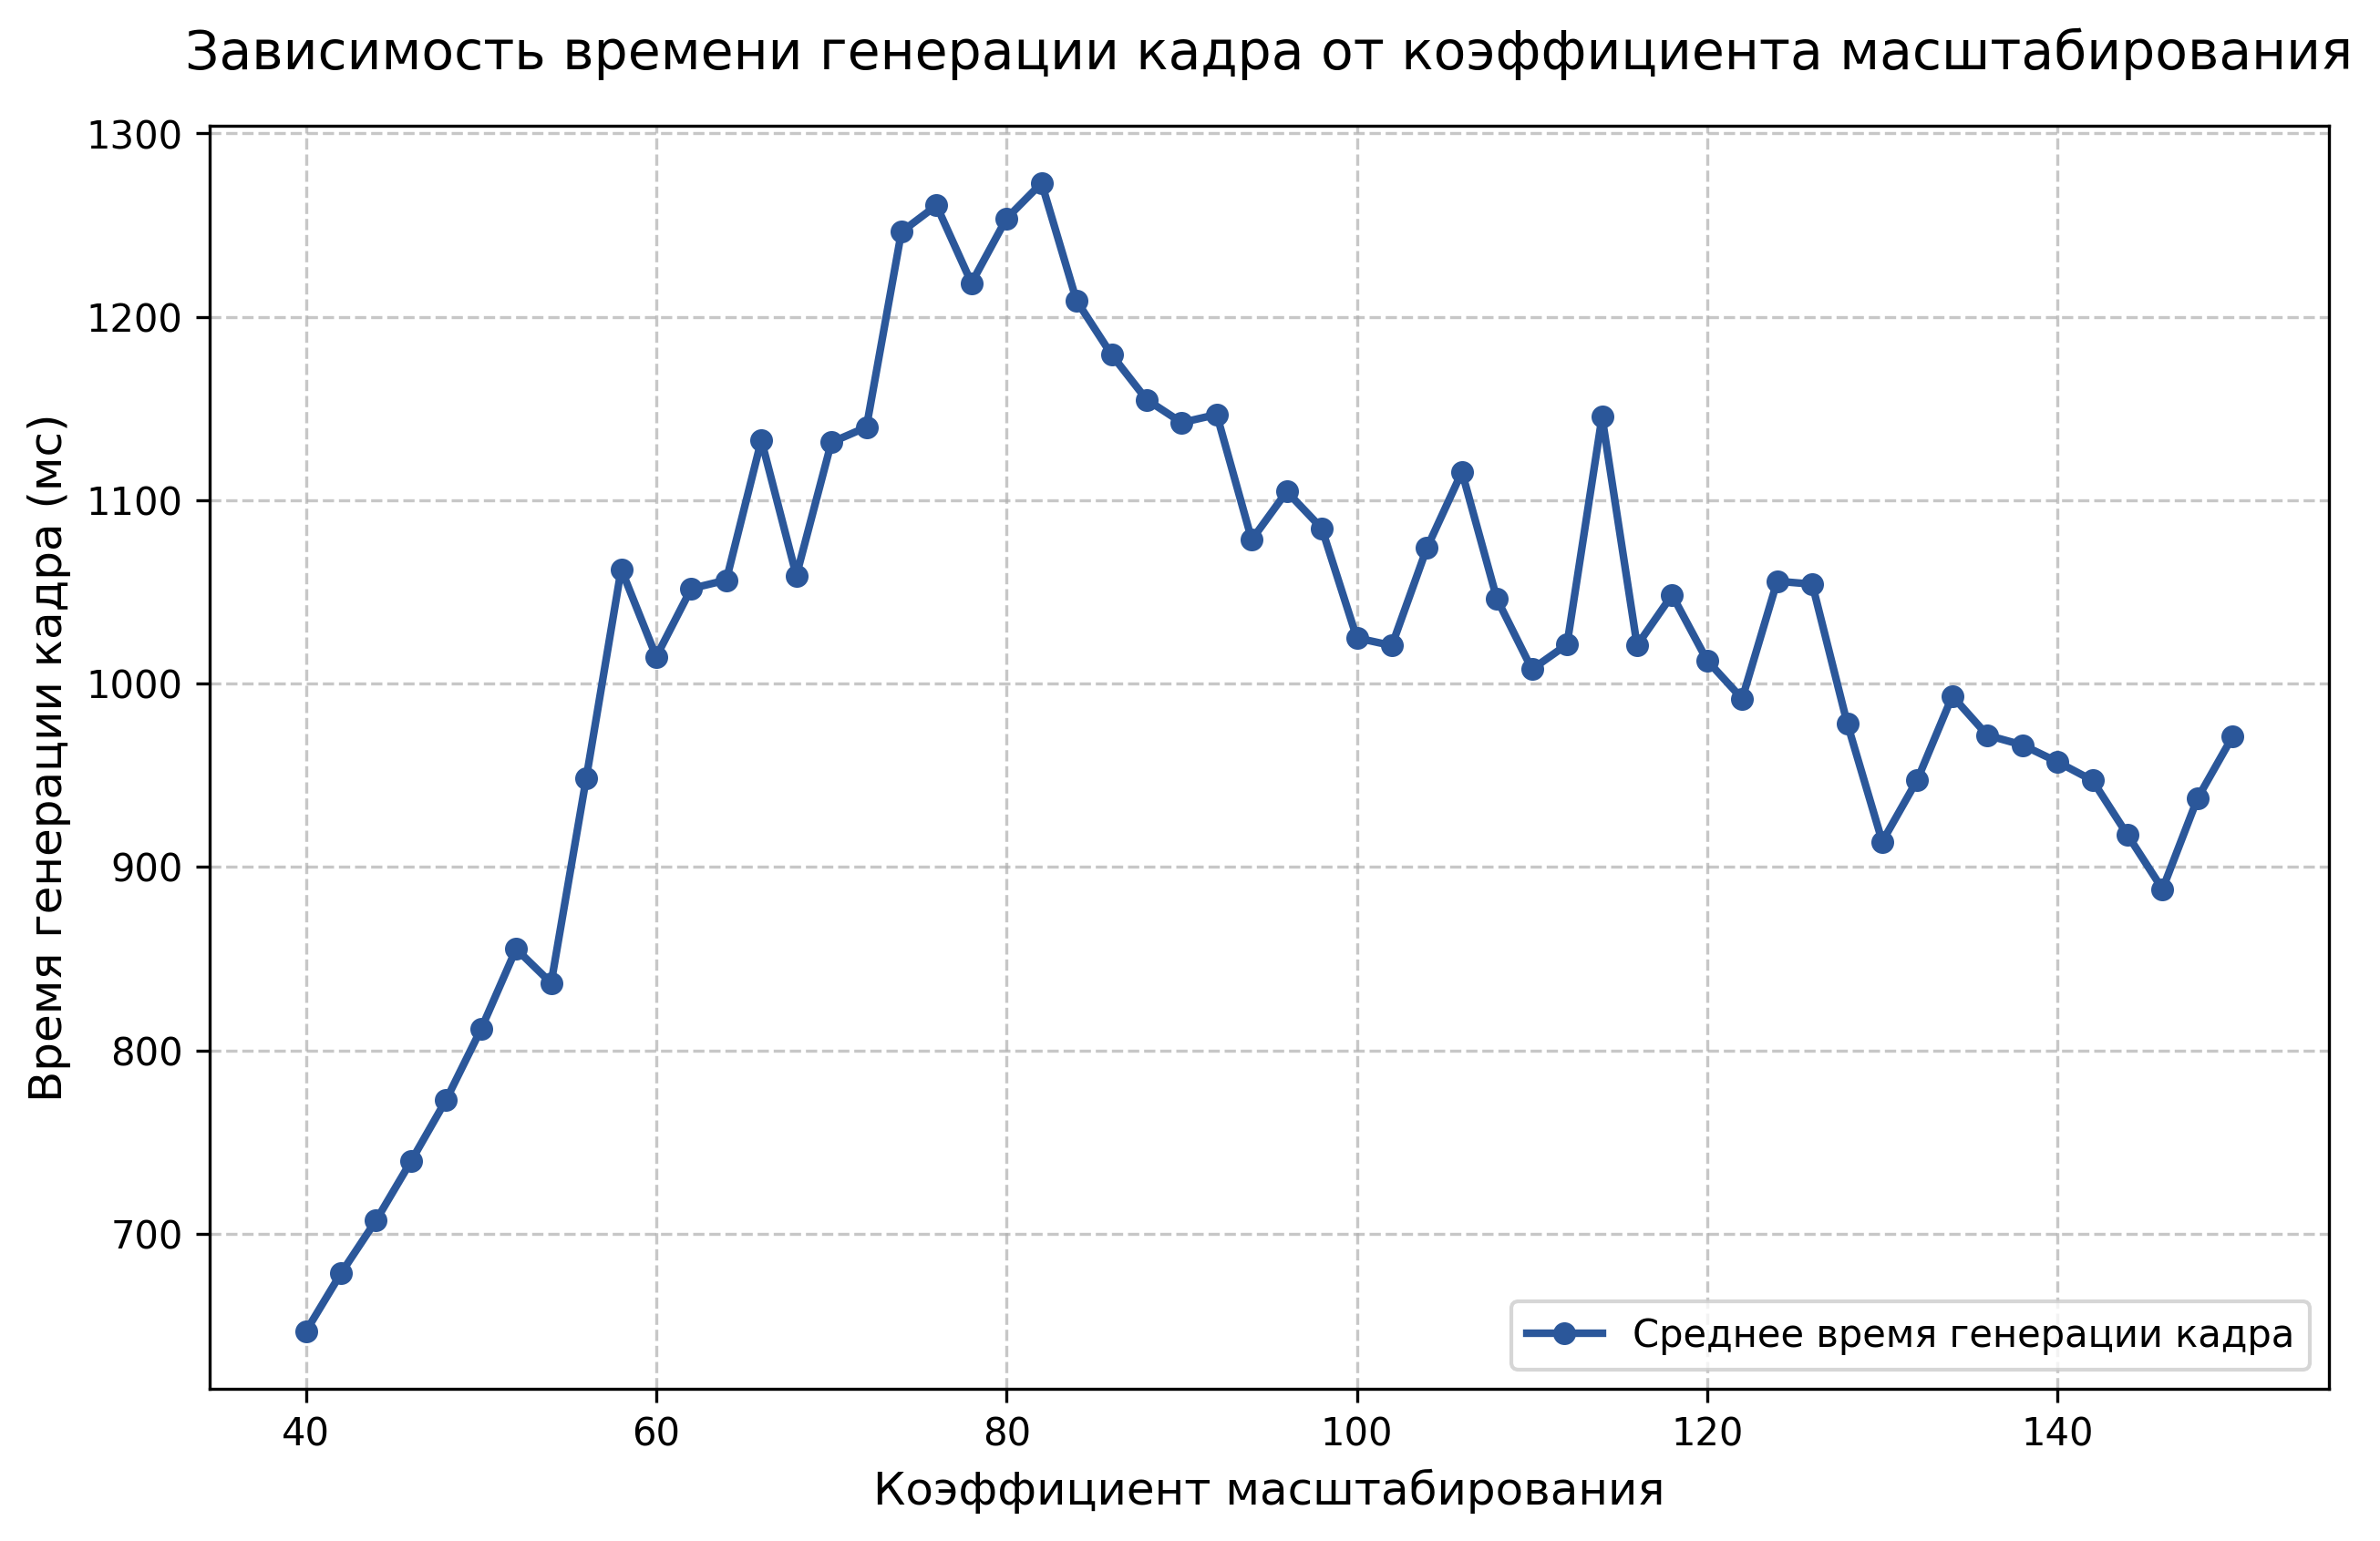
\includegraphics[width=0.9\textwidth]{img/research_graph}
	\caption{График зависимости времени генерации кадра от коэффициента масштабирования}
	\label{fig:research_graph}
\end{figure}

\section{Анализ результатов}

На основании полученных данных можно выделить характерные этапы изменения производительности, которые объясняются особенностями работы алгоритма построчного сканирования (Scanline Z-Buffer).

\begin{enumerate}
	\item\textbf{Рост нагрузки (Scale 40.0 $\to$ 82.0).}
	В диапазоне масштабов от 40 до 82 наблюдается рост времени рендеринга с 646,8 мс до пикового значения 1272,9 мс. Это связано с тем, что при увеличении масштаба объекты сцены занимают всё большую площадь экрана. Поскольку алгоритм работает на CPU, его производительность ограничена скоростью заполнения пикселей.
	
	\item\textbf{Пик нагрузки (Scale $\approx$ 82.0).}
	Максимальное время генерации кадра 1272,9 мс достигается при коэффициенте масштабирования 82.0. В этот момент сцена максимально заполняет видимую область экрана, но объекты еще практически не выходят за его границы. Процессор вынужден обрабатывать и закрашивать максимальное количество пикселей для всей геометрии сцены.
	
	\item\textbf{Спад нагрузки и стабилизация (Scale > 82.0).}
	При дальнейшем увеличении масштаба (от 82 до 150) крупные объекты начинают выходить за границы кадра. В этот момент в алгоритме растеризации срабатывает механизм \textbf{отсечения (Clipping)}. Полигоны или их части, координаты которых находятся вне области видимости ($X < 0$ или $X > Width$), отбрасываются. Это снижает нагрузку на процессор, и время рендеринга снижается, стабилизируясь в диапазоне \textbf{900–1000 мс}.
\end{enumerate}

\section{Выводы по исследовательской части}

Проведенный эксперимент позволил сделать выводы о работе разработанной систем.

\begin{enumerate}
	\item Фактором, ограничивающим производительность, является количество пикселей сцены, которые в данный момент отображаются на экране. Приближение камеры увеличивает нагрузку до тех пор, пока объекты полностью помещаются в кадр.
	\item Реализованный механизм отсечения и векторизация вычислений работают: при выходе объектов за границы кадра время рендеринга уменьшается, несмотря на то, что математически объекты становятся крупнее.
	\item Система демонстрирует стабильную работу с FPS около 0.8–1.5 на сложной сцене с тенями в высоком разрешении ($1200 \times 1200$) на центральном процессоре.
\end{enumerate}